\chapter{基于维基百科的概念属性生成}
\label{cha:concept-property}

\section{本章引论}

本体构建中,Taxonomy作为骨架,占有重要地位。Taxonomy包含本体的概念与属性,属性为概念下一类实例的共有特性。

为了获取通用领域下概念与属性的关系,本章中,我们对维基百科进行了详细地观察与解析,获得了维基中模板与属性的规则。

维基百科鼓励编辑者使用模板对词条以及信息框进行组织与编辑。模板是百科针对不同主题的词条内容所列出的标准结构框架,类似于长期积累形成的标准写作规范。模板使词条的结构变得有规律可循,也可以有效避免关键信息的缺失。信息框的编辑也可模板化,信息框模板包含了描述一类实例的常用属性。图\ref{fig:template-infobox-film}为\textit{Template:电影信息框(Template:Infobox Film)}\footnote{https://zh.wikipedia.org/wiki/Template:电影信息框},其中含有电影的诸多属性,如\textit{演员,导演,时长}等。模板在一定程度上描述了一个领域的信息,充分利用其中信息,对概念-属性关系的研究有很大意义。

本文主要对信息框属性进行研究,后文中提到的模板,同一指代{\heiti 信息框模板}。

\begin{figure}[H]
  \centering
  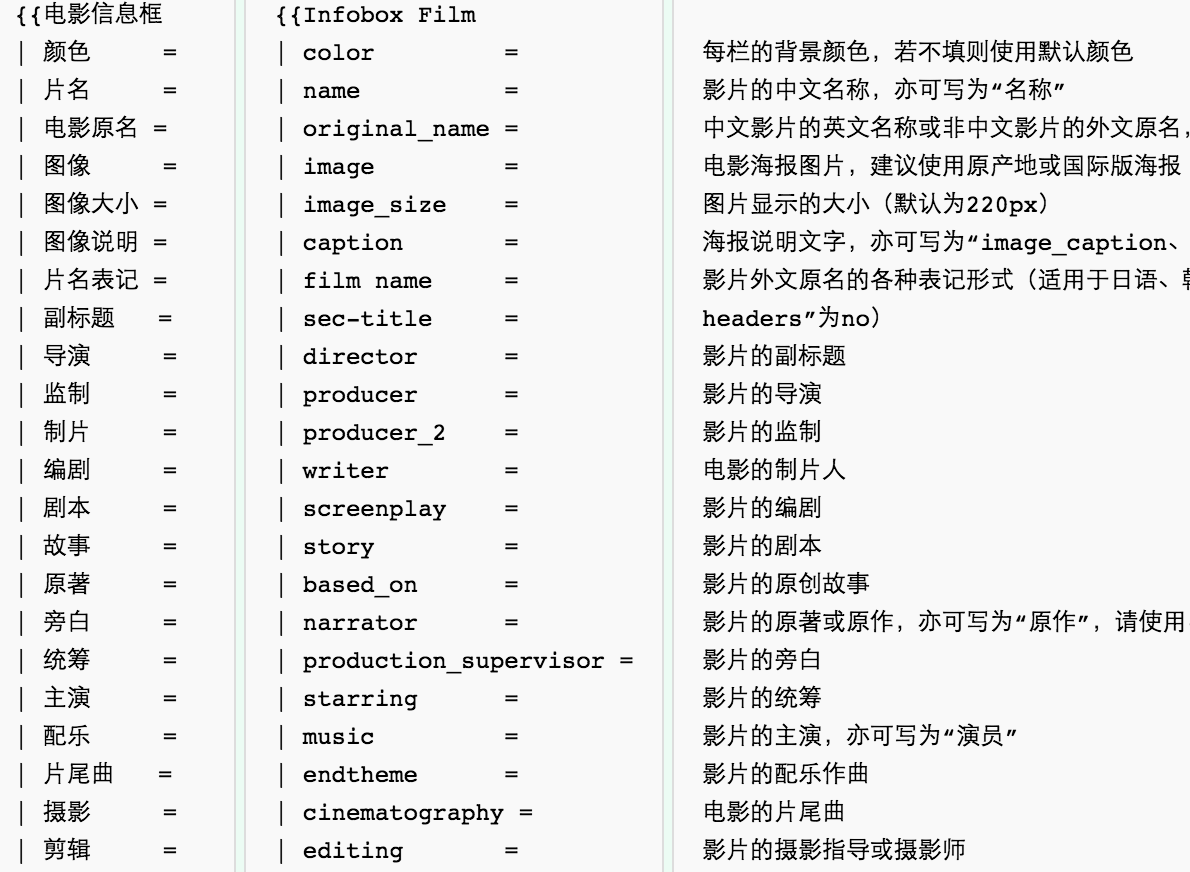
\includegraphics[width=0.8\columnwidth]{template-infobox-film}
  \caption{电影信息框模板}
  \label{fig:template-infobox-film}
\end{figure}

基于对模板设计的思考,我们提出概念属性:即概念下有特定的属性集合对实例进行描述,属性的定义依赖于概念,不同概念下的属性意义可能不一样。以领域信息区分属性,有助于避免属性歧义问题。同时,考虑到维基信息框模板规范着一个概念下对实例的描述,我们可以用{\heiti 属性@模板}定义一个属性。

因为百科数据杂乱,概念属性生成的工作繁琐但至关重要,结果的数量与质量,在很大程度上影响着其他属性研究的准确率,过多杂质的引入会增加相关工作的难度。

本章工作充分利用维基百科的结构化信息,从中英文数据文件中,提取概念属性,其结果覆盖了90\%以上的维基词条,为今后对信息框属性的进一步分析打下了良好的基础。

\section{维基百科信息框模板与属性分析}
\label{sec:template-analysis}

维基百科自2001年创立,经过15年左右的发展,不仅储备了海量数据,在编辑规则上也越发规范。但因为词条繁杂、参与人数众多,还是无法保证数据统一,质量差强人意,这使生成概念属性的工作困难重重。

具体来说,维基所提供的数据文件\footnote{https://dumps.wikimedia.org}中,词条信息框的内容是以{\heiti 模板标签}来组织的,而模板标签与真正展示在网页上的{\heiti 显示标签}不同。模板标签与显示标签的关系在对应语言的信息框模板词条下有定义。图\ref{fig:film-tl-rl},电影\textit{疯狂动物城}的配乐为\textit{迈克尔·吉亚奇诺},这条信息在词条中的数据文件中是\textit{music=[[麥可·吉亞奇諾]]},而在网页中的显示是\textit{配乐作曲 \ 迈克尔·吉亚奇诺},其中,\textit{music}为模板标签,\textit{配乐作品}为显示标签,而两种标签的对应关系,在词条\textit{Template:电影信息框}中有所说明(见图\ref{fig:template-infobox-film})。维基百科的这种设计,使模板属性在不同语言上有了标准规范。对于任意一个语言,在设计自己的电影信息框模板时,只需根据模板标签,给出对应的显示标签即可,对多语言百科来说,不失为一种好方法。但是间接获得显示标签,也对模板的获取增加了难度,而人为设计的不规范性,又雪上加霜。

\begin{figure}[H]
  \centering
  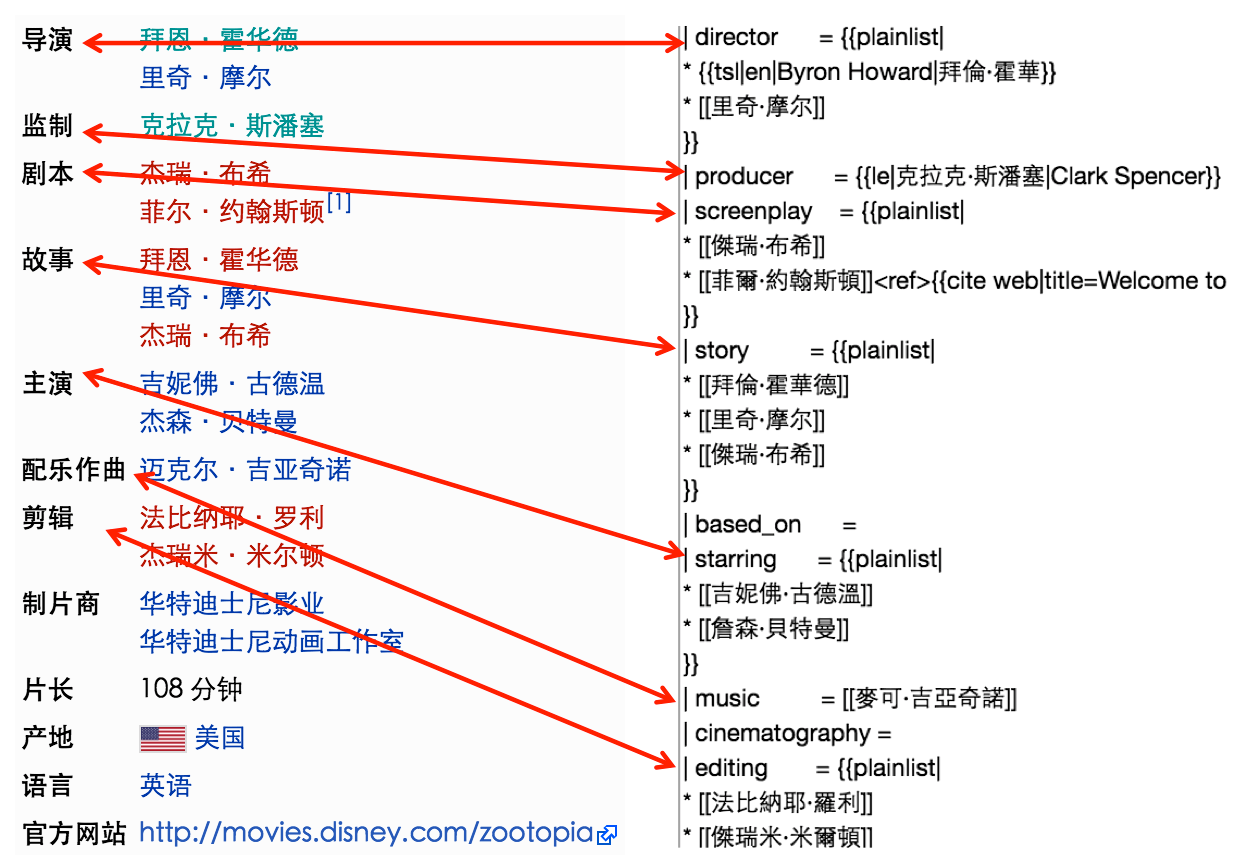
\includegraphics[width=0.8\columnwidth]{film-tl-rl}
  \caption{电影《疯狂动物城》模板标签与显示标签对比}
  \label{fig:film-tl-rl}
\end{figure}

而真实的模板是怎么定义的呢?模板在维基百科中也设计成一个词条,在维基article数据文件中,含有对模板词条的具体定义。模板词条标签以\textit{Template:}开头,大部分的信息框模板标签则以\textit{Template:Infobox}开头,但也有例外,在中文维基中,类似\textit{Template:电影信息框}等具有语言本地化特色的标签有很多。在之后的工作中,我们统计出以\textit{Template:Infobox}标识的模板占所有英文信息框模板的91\%,中文的63.5\%。由此可见,单纯通过词条标签来筛选出信息框模板并不是一个良策。

通过对模板内容进行总结,我们发现信息框模板的源代码中都含有\textit{infobox}字样,该infobox所涵盖的区域中,包含模板属性定义,可以认为带有infobox信息的Template为信息框模板。

尽管区分出信息框模板,模板中内容格式却不尽相同。根据版式特点,我们将信息框模板归为三类,分别为键值对模板、表格模板与继承模板,图\ref{fig:template-examples}给出三种模板示例,我们将在\ref{sec:property-extraction}中给出详细介绍。

\begin{figure}[h]
  \caption{模板类型举例}
  \label{fig:template-examples}

  \begin{subfigure}{3cm}
    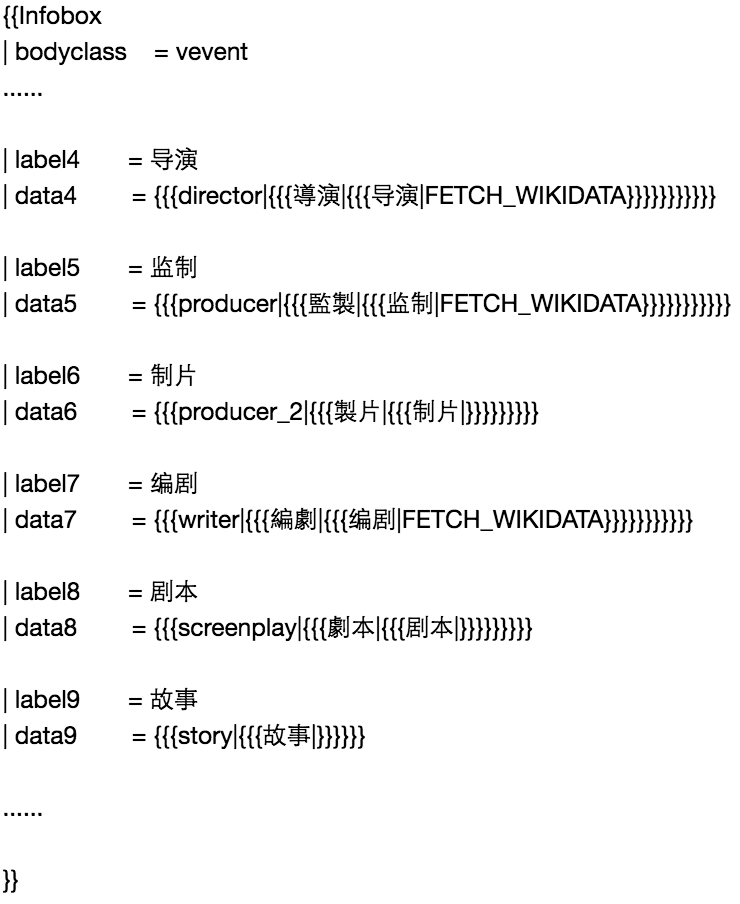
\includegraphics[height=3cm]{template-keyvalue}
    \caption{键值对模板示例}
  \end{subfigure}%
  \hspace{4em}%

  \begin{subfigure}{3cm}
    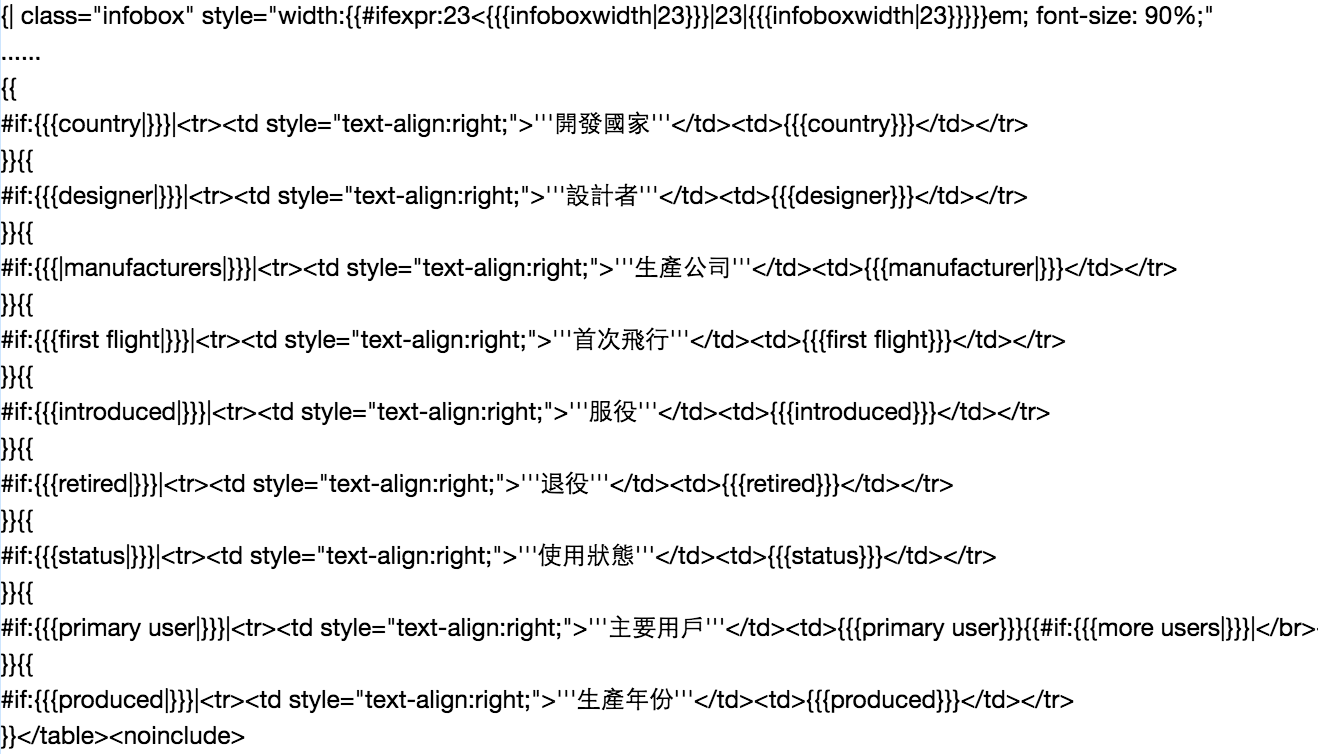
\includegraphics[height=3cm]{template-table}
    \caption{表格模板示例}
  \end{subfigure}%
  \hspace{4em}%

  \begin{subfigure}{3cm}
    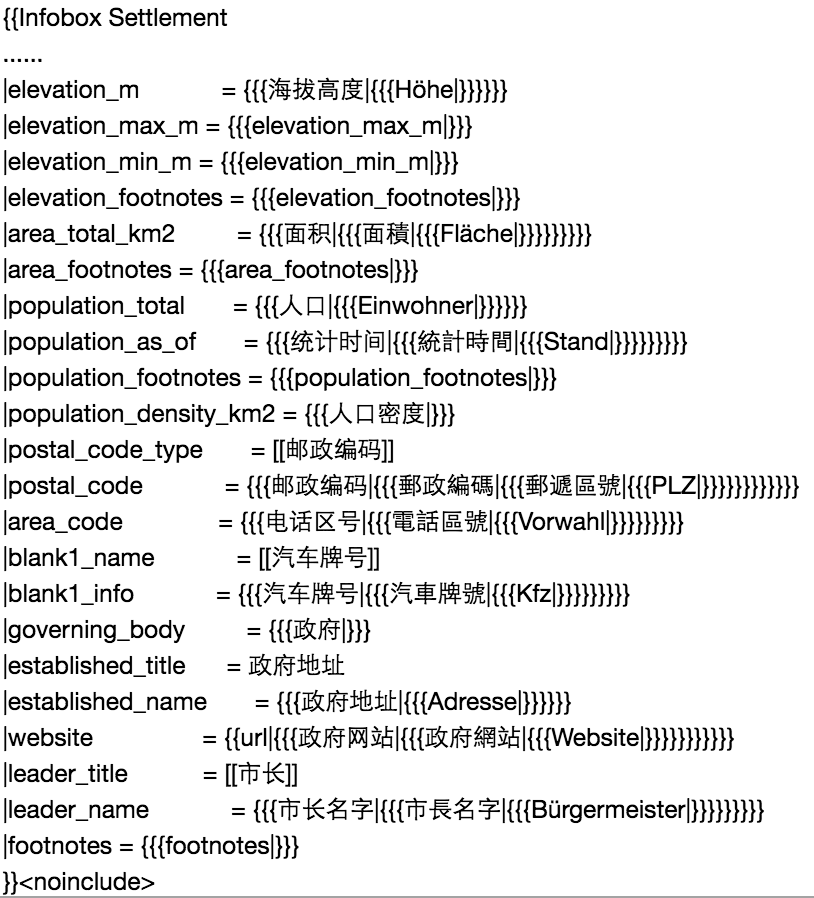
\includegraphics[height=3cm]{template-inherit}
    \caption{继承模板示例}
  \end{subfigure}%
\end{figure}

除了以上三类,数据文件中还出现了{\heiti 重定向模板},内容如图\ref{fig:template-redirect}。该类模板的出现,是因为维基百科经过多次整理与更新,会将相似模板合并,或重新定义模板名称,被删除的模板会重定向到新模板上。2016年2月的中文维基上,\textit{Template:Infobox Film}与\textit{Template:Infobox film}都重定向到\textit{Template: 电影信息框}。

\begin{figure}[H]
  \centering
  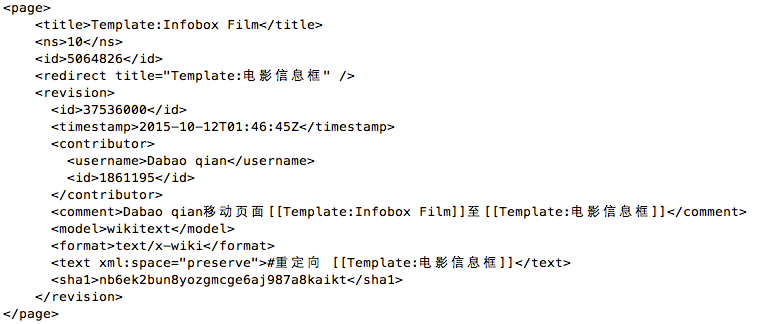
\includegraphics[width=0.7\columnwidth]{template-redirect}
  \caption{重定向模板内容展示}
  \label{fig:template-redirect}
\end{figure}

\section{问题描述}

我们认为,一个指定的概念$c_i \in C$所代表的领域下,会有一个属性集合$P(c_i)=\{p_{i,j}|j=1,2,...,n\}$表征$c_i$中的所有实例$I(c_i)$的特性。我们定义概念属性$p_{c_i}= <c_i, label, I, V>$,表示其带有概念$c_i$的领域信息,只描述$i_{c_i} \in I(c_i)$。$label$表示属性标签,即使$p_{c_i}.label == p_{c_j}.label$,$p_{c_i} \neq p_{c_j}$。$I$代表$p_{c_i}$在$c_i$下描述的实例集合,$V$代表$p_{c_i}$的描述$I$的所有值集合。

本章的工作是从维基百科中生成概念属性。给定一个维基百科$W$,可以得到模板$T$,模板存储描述一类实例的属性集合,对于模板$t_i$,我们有$P(t_i)=\{p_{i,j}|j=1,2,...,n\}$。可以认为,模板代表着一类概念,则有$T \approx C$。

鉴于\ref{sec:template-analysis}中对模板与属性的分析,基于维基的概念属性,在定义上需要进行一些改动:
\begin{itemize}
\item 维基百科在数据文件中使用的属性标签,与现实在页面的不一致(图\ref{fig:film-tl-rl})。我们将数据文件中使用的标签定义为模板标签(template label),用$tl$表示,展示在页面上的称为显示标签(render label),用$rl$表示。则有$p_{c_i}.label = <tl, rl>$。
\item 维基百科的模板可能有相近或重复,此时所代表的概念是存在包含关系的。因此严格来说,有$c = \{t_i|i=1,2...n\}$。
\end{itemize}

具体到维基百科,本章工作抽象为:给定一个维基百科$W = <T>$,生成概念集合$C$,其中$c = \{t_i|i=1,2...n\}, c \in C, t_i \in T$,以及概念属性集合$\Rho = \{P(c_i)| i = 1,2,...,n\}$,其中对于$p_{c_i} \in P_{c_i}$,有$p_{c_i} = <c_i, tl, rl>$。

\section{概念属性生成}
\label{sec:property-extraction}

我们对三类信息框模板分别进行抽取,收集模板标签与显示标签的关系。我们发现,一个属性的显示标签,可能根据模板标签有所变化。抽取过程中,所有模板标签与显示标签的关系都会保留下来,我们以$<T, tl, rl>$的格式保留一组属性记录。

{\heiti 键值对模板($T_{kv}$)(图\ref{fig:template-examples}a):} 这种类型的模板,其显示标签与模板标签在infobox中以

\begin{figure*}[ht]
\begin{center}
\framebox[0.4\linewidth]{
    \begin{minipage}[t]{0.25\linewidth}
    \ label=显示标签\\
    \ data=模板标签 
    \end{minipage}
}
\end{center}
\end{figure*}

的格式存在。一个模板中,显示标签与模板标签的关系可能是一对一、一对多、多对多的,即一个属性根据不同的模板标签,可能会显示不同的标签在页面上。

{\heiti 表格模板($T_{table}$)(图\ref{fig:template-examples}b):}这种类型的模板以类似表格的形式对属性进行编排,抽取方法与键值对模板不同,根据表格行列思想,通过分析<td>等标签抽取。

{\heiti 继承模板($T_{inherit}$)(图\ref{fig:template-examples}c):}有半数左右的模板存在继承关系,即其模板标签的表示含义与父类模板相同,标签对应关系要结合父类模板来挖掘。继承模板可能继承自键值对模板、表格模板,甚至重定向模板。

{\heiti 重定向模板($T_{redirect}$)(图\ref{fig:template-redirect}):}对于分析实例对模板的应用情况至关重要,编辑者可能在编写信息框时用的旧版模板标签,或者不注意大小写。\ref{fig:template-redirect-examples}给出不同词条对同一模板的不同编辑方式。如果不考虑重定向模板标签,在前三类的基础上直接匹配,会大大影响已抽取模板对词条的覆盖率。因此重定向模板虽然没有实质内容,也不能弃之不理。

\begin{figure}[H]
  \centering
  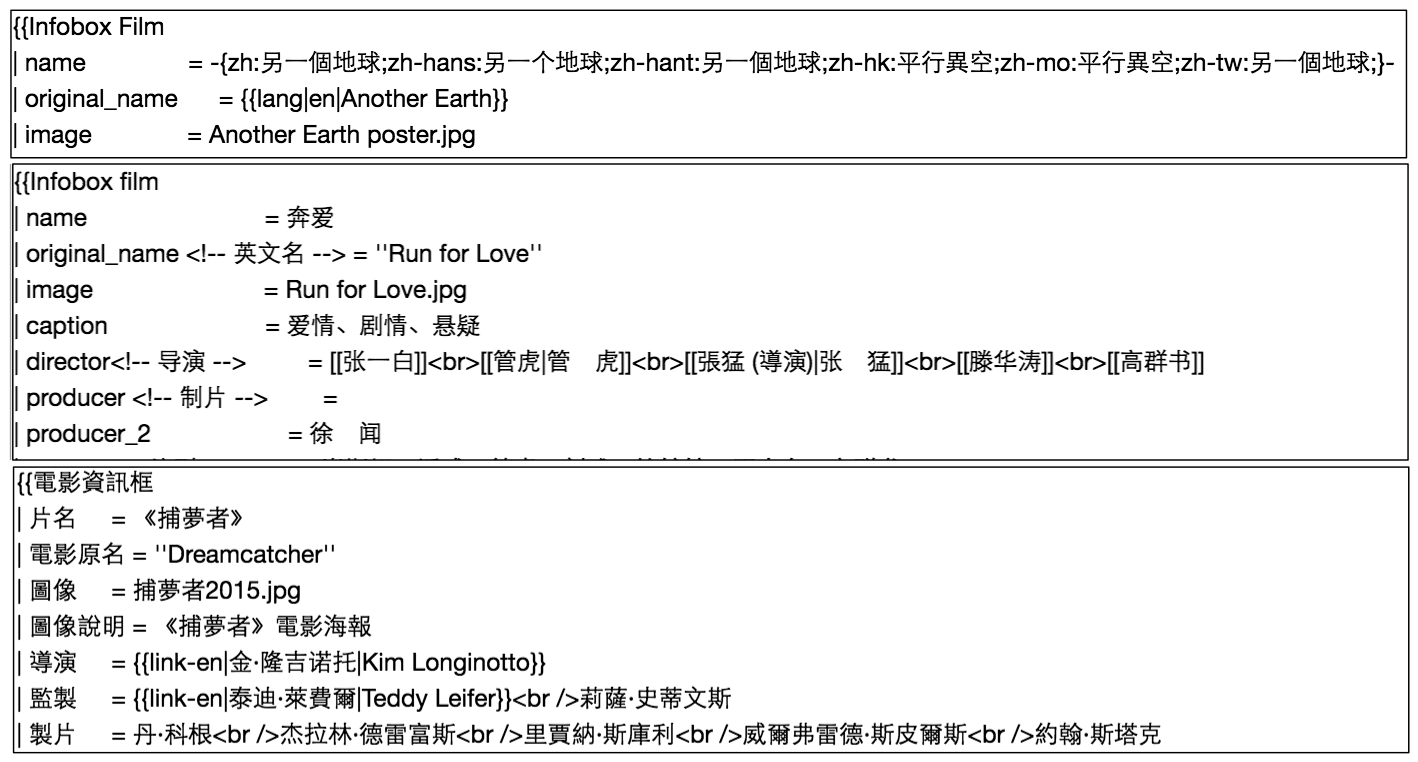
\includegraphics[width=0.8\columnwidth]{template-redirect-examples}
  \caption{重定向模板使用情况举例}
  \label{fig:template-redirect-examples}
\end{figure}

\subsection{结果统计}

基于以上四类信息框模板,我们对2016.03版本的英文维基与2016.02版本的中文维基分别抽取,表\ref{tab:wiki-infobox-statistic}是对当前维基现状的统计分析。

\begin{table}[htb]
  \centering
  \caption{中英文维基百科词条信息统计}
  \label{tab:wiki-infobox-statistic}
  \begin{minipage}[t]{1\textwidth} 
    \begin{tabularx}{\linewidth}{lXXX}
      {\heiti 维基百科} & {\heiti \#词条} &  {\heiti \#含有信息框词条} & {\heiti \#被使用模板} \\\midrule[1pt]
      英文维基 & 5,138,426 & 2,344,305(45.6\%) & 4491 \\
      中文维基 & 863,918   & 261,045(30.2\%)   & 2317  \\
      \bottomrule[1.5pt]
    \end{tabularx}
  \end{minipage}
\end{table}

得到各类型信息框模板数量如表\ref{tab:infobox-template}所示

\begin{table}[htb]
  \centering
  \caption{各类型信息框模板数量}
  \label{tab:infobox-template}
  \begin{minipage}[t]{1\textwidth} 
    \begin{tabularx}{\linewidth}{lXXXXX}
      {\heiti 维基百科} & {\heiti \#$T_{kv}$} &  {\heiti \#$T_{table}$} & {\heiti \#$T_inherit$} & {\heiti \#$T_redirect$} & {\heiti 总数}\\\midrule[1pt]
      英文维基 & 1910 & 1901 & 1897 & 4076 & 9784\\
      中文维基 & 840  & 878  & 968  & 956  & 3642\\
      \bottomrule[1.5pt]
    \end{tabularx}
  \end{minipage}
\end{table}

我们对各模板进行了分析,因为数据杂乱等原因,我们无法成果获取所有模板中的信息,而是以常用模板为优先,并以词条覆盖率90\%以上为目标结束属性生成任务。成功解析的属性信息如表\ref{tab:render-label}所示,其中不包括对重定向模板的解析。

\begin{table}[htb]
  \centering
  \caption{概念属性信息生成结果}
  \label{tab:render-label}
  \begin{minipage}[t]{1\textwidth} 
    \begin{tabularx}{\linewidth}{lXXXX}
      {\heiti 维基百科} & {\heiti \#$T$} & {\heiti \#模板属性} & {\heiti 属性/模板}  &{\heiti 模板标签/属性} \\\midrule[1pt]
      英文维基 & 3819 & 104741 & 27.45 & 1.27  \\
      中文维基 & 1895 & 44797  & 23.64 & 1.34  \\
      \bottomrule[1.5pt]
    \end{tabularx}
  \end{minipage}
\end{table}

我们在\ref{tab:coverage}中给出当前生成的概念属性对维基百科的覆盖程度。实际使用的模板名称与模板正式名称的匹配率较低,需要经过一系列转化,包括:大小写转换、去除多余空格、重定向模板转换等。
模板覆盖率为抽取出的模板数量与所有词条使用的全部模板数量的占比,模板属性覆盖率为所有抽取出的模板属性对所有词条的所有属性数量的占比,词条覆盖率为能用抽取模板分析的词条的百分比,我们获取的概念属性可以处理90\%以上的维基词条的信息框。

\begin{table}[htb]
  \centering
  \caption{结果覆盖率统计}
  \label{tab:coverage}
  \begin{minipage}[t]{1\textwidth} 
    \begin{tabularx}{\linewidth}{lXXX}
      {\heiti 维基百科} & {\heiti 模板覆盖率}  {\heiti 模板属性覆盖率}  & {\heiti 词条覆盖率} \\\midrule[1pt]
      英文维基 & 87.6\% & 27\% & 96.7\%  \\
      中文维基 & 77.8\% & 33\% & 90.3\%  \\
      \bottomrule[1.5pt]
    \end{tabularx}
  \end{minipage}
\end{table}

%\section{概念合并}
%
%最后我们有xx个概念,共xx个属性
%
\section{本章小结}

本章主要从维基百科中生成概念属性。我们将维基模板相关的领域视为概念,其中的属性视为该概念下的属性,并用\textit{属性@模板}的方式定义一个属性,这种方法同时可以解决属性多义问题,即认为同一领域下的属性没有歧义性。

为了获得尽可能多的概念属性,我们对维基百科模板和属性进行了细致的分析,将模板分为键值对模板、表格模板、继承模板与重定向模板,分别进行处理,将属性赋予模板标签与显示标签两种信息,这些工作,有助于他人对于属性和模板有更深入的理解。

